\section{Auswertung}
\label{sec:Auswertung}
\subsection{Fourieranalyse}
Es werden die ersten 9 von null verschiedenen Fourieramplituen einer Rechteck-,
Sägezahn- und Dreiecksschwinung gemessen.
In Abbildung \ref{fig:linienspektrum_rechteck} ist das Linienspektrum der
Rechteckschwingung zu sehen. Die daraus abgelesenen Werte der Amplituden sind in
Tabelle \ref{tab:analyse_rechteck} dargestellt. Desweiteren sind in der Tabelle
die Theoriewerte der Fourieramplituden eingetragen und der relative Fehler
zwischen Theorie- und Messwert.
Der relative Fehler berechnet sich dabei nach
\begin{equation}
  \Delta x_\symup{rel} = \left|\frac{x_\text{t} - x_\text{m}}
  {x_\text{t}} \right|.
  \label{eqn:relativer_fehler}
\end{equation}
Die Fourierkoeffizienten sind nach der Berechnung in Abschnitt \ref{sec:Rechteckspannung}
proportional zu $\frac{1}{n}$. Die Theoriewerte ergeben sich daher aus
\begin{equation}
  a_\symup{n} = \frac{a_1}{n}.
  \label{eqn:a_n_rechteck}
\end{equation}

\subsubsection{Rechteckschwingung}
Für die Rechteckschwingung gilt $a_1 = 4.24 \si{\volt}$.
\begin{figure}
  \centering
  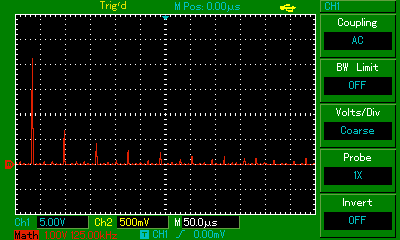
\includegraphics[width=0.7\textwidth]{linienspektrum_rechteck.png}
  \caption{Linienspektrum einer Rechteckschwingung.}
  \label{fig:linienspektrum_rechteck}
\end{figure}

\begin{table}
  \centering
  \begin{tabular}{c c c c}
    \toprule
    Oberwelle & $U_\text{m}$ in \si{\volt} & $U_\text{theo}$ in \si{\volt} &
    relative Abweichung in \% \\
    \midrule
    1  & 4.24  & 4.24  & 0.00 \\
    3  & 1.38  & 1.41  & 2.12 \\
    5  & 0.864 & 0.848 & 1.89 \\
    7  & 0.572 & 0.606 & 5.61 \\
    9  & 0.488 & 0.471 & 3.61 \\
    11 & 0.348 & 0.385 & 9.61 \\
    13 & 0.336 & 0.326 & 3.07 \\
    15 & 0.252 & 0.282 & 10.6 \\
    17 & 0.160 & 0.249 & 35.7 \\
    \bottomrule
  \end{tabular}
  \caption{Vergleich von gemessenen und berechneten Werten für die Amplituden
    der Koeffizienten bei der Analyse der Rechteckschwingung.}
  \label{tab:analyse_rechteck}
\end{table}

\subsubsection{Sägezahnschwingung}
In Abbildung \ref{fig:linienspektrum_saegezahn} ist nun das Linienspektrum der
Sägezahnschwingung zu sehen. Die daraus abgelesenen Werte der Amplituden sind in
Tabelle \ref{tab:analyse_saegezahn} dargestellt. Zusätzlich sind in der Tabelle
wieder die Theoriewerte der Fourieramplituden eingetragen und der relative Fehler
zwischen Theorie- und Messwert.
Auch hier sind die Fourierkoeffizienten nach der Berechnung in Abschnitt \ref{sec:Saegezahnspannung}
proportional zu $\frac{1}{n}$ und die Theoriewerte werden daher nach Gleichung
\eqref{eqn:a_n_rechteck} berechnet. Für Die Sägezahnschwingung gilt $a_1 = 2.14
\si{\volt}$.

\begin{figure}
  \centering
  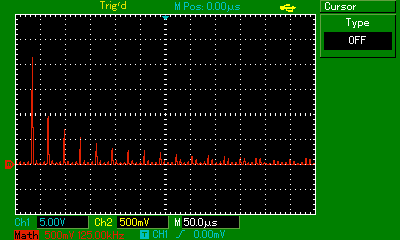
\includegraphics[width=0.7\textwidth]{linienspektrum_saegezahn.png}
  \caption{Linienspektrum einer Sägezahnschwingung.}
  \label{fig:linienspektrum_saegezahn}
\end{figure}

\begin{table}
  \centering
  \begin{tabular}{c c c c}
    \toprule
    Oberwelle & $U_\text{m}$ in \si{\volt} & $U_\text{theo}$ in \si{\volt} &
    relative Abweichung in \% \\
    \midrule
    1 & 2.14  & 2.14  & 0.00 \\
    2 & 0.968 & 1.07  & 9.53 \\
    3 & 0.696 & 0.713 & 2.38 \\
    4 & 0.552 & 0.535 & 3.18 \\
    5 & 0.436 & 0.428 & 1.87 \\
    6 & 0.332 & 0.357 & 7.00 \\
    7 & 0.292 & 0.306 & 4.57 \\
    8 & 0.272 & 0.268 & 1.49 \\
    9 & 0.240 & 0.238 & 0.84 \\
    \bottomrule
  \end{tabular}
  \caption{Vergleich von gemessenen und berechneten Werten für die Amplituden
    der Koeffizienten bei der Analyse der Sägezahnschwingung.}
  \label{tab:analyse_saegezahn}
\end{table}

\newpage
\subsubsection{Dreiecksschwingung}
Zuletzt ist in Abbildung \ref{fig:linienspektrum_saegezahn} das Linienspektrum der
Dreiecksschwingung zu sehen. Die daraus abgelesenen Werte der Amplituden sind in
Tabelle \ref{tab:analyse_saegezahn} dargestellt. Wie zuvor sind in der Tabelle
die Theoriewerte der Fourieramplituden eingetragen und der relative Fehler
zwischen Theorie- und Messwert.
Hier sind die Fourierkoeffizienten nach der Berechnung in Abschnitt \ref{sec:Dreieckspannung}
proportional zu $\frac{1}{n^2}$. Die Berechnung der Theoriewerte erfolgt daher mit
\begin{equation}
  a_\symup{n} = \frac{a_1}{n^2}.
  \label{eqn:a_n_dreieck}
\end{equation}
Bei der Dreiecksschwingung ist $a_1 = 2.72 \si{\volt}$.

\begin{figure}
  \centering
  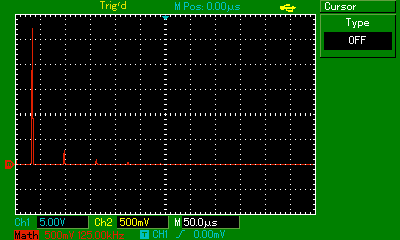
\includegraphics[width=0.7\textwidth]{linienspektrum_dreieck.png}
  \caption{Linienspektrum einer Dreiecksschwingung.}
  \label{fig:linienspektrum_dreieck}
\end{figure}

\begin{table}
  \centering
  \begin{tabular}{c c c c}
    \toprule
    Oberwelle & $U_\text{m}$ in \si{\volt} & $U_\text{theo}$ in \si{\volt} &
    relative Abweichung in \% \\
    \midrule
    1  & 2.72  & 2.72  & 0.00 \\
    3  & 0.300 & 0.302 & 0.66 \\
    5  & 0.111 & 0.109 & 1.83 \\
    7  & 0.052 & 0.055 & 5.45 \\
    9  & 0.035 & 0.034 & 2.94 \\
    11 & 0.021 & 0.022 & 4.54 \\
    13 & 0.016 & 0.016 & 0.00 \\
    15 & 0.012 & 0.012 & 0.00 \\
    17 & 0.007 & 0.009 & 22.2 \\
    \bottomrule
  \end{tabular}
  \caption{Vergleich von gemessenen und berechneten Werten für die Amplituden
    der Koeffizienten bei der Analyse der Dreieckschwingung.}
  \label{tab:analyse_dreieck}
\end{table}


\subsection{Fouriersynthese}
Nun werden die Spannungsamplituden der einzelnen Oberwellen für drei verschiedene
Schwingungen (Rechteck-, Sägezahn- und Dreiecksschwingung) so eingestellt, dass
die Fouriersynthese die gewünschte Schwingungsform liefert. Dazu werden die ersten
neun Oberwellen verwendet.
Die Summenschwingung wird mit einem Oszilloskop betrachtet. Die durch die
Fouriersynthese entstandene Schwingungen sind in den Abbildungen
\ref{fig:rechteck_synthese}, \ref{fig:saegezahn_synthese} und \ref{fig:dreieck_synthese}
abgebildet. In den Tabellen \ref{tab:synthese_rechteck}, \ref{tab:synthese_saegezahn}
und \ref{tab:synthese_dreieck} sind die Fourieramplituen, die theoretisch
einzustellen gewesen wären, sowie die tatsächlich eingestellten Amplituden für die
jeweilige Fouriersynthese dargestellt. Die Abweichungen entstanden, da die Regler
für die Amplitude nicht genauer einzustellen waren.

\newpage
\subsubsection{Rechteckschwingung}
\begin{figure}
  \centering
  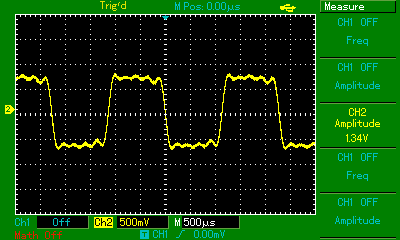
\includegraphics[width=0.7\textwidth]{rechteck.png}
  \caption{Synthetisierte Rechteckschwingung.}
  \label{fig:rechteck_synthese}
\end{figure}
\begin{table}
  \centering
  \begin{tabular}{c c c c}
    \toprule
    Oberwelle & $U_\text{e}$ in \si{\volt} & $U_\text{theo}$ in \si{\volt} &
    relative Abweichung in \% \\
    \midrule
    1 & 1.76  & 1.76  & 0.00 \\
    3 & 0.574 & 0.587 & 2.21 \\
    5 & 0.356 & 0.352 & 1.14 \\
    7 & 0.257 & 0.251 & 2.39 \\
    9 & 0.198 & 0.196 & 1.02 \\
    \bottomrule
  \end{tabular}
  \caption{Vergleich von eingestellten und berechneten Werten für die Amplituden
    der Koeffizienten bei der Synthese der Rechteckschwingung.}
  \label{tab:synthese_rechteck}
\end{table}

\newpage
\subsubsection{Sägezahnschwingung}
\begin{figure}
  \centering
  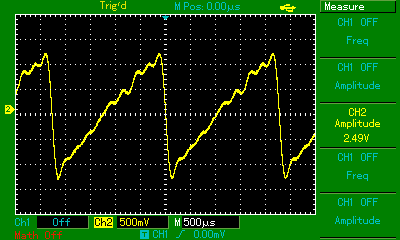
\includegraphics[width=0.7\textwidth]{saegezahn.png}
  \caption{Linienspektrum einer Sägezahnschwingung.}
  \label{fig:saegezahn_synthese}
\end{figure}
\begin{table}
  \centering
  \begin{tabular}{c c c c}
    \toprule
    Nummer der Oberwelle & $U_\text{e}$ in \si{\volt} &
    $U_\text{theo}$ in \si{\volt} & relative Abweichung in \% \\
    \midrule
    1 & 1.76  & 1.76  & 0.00 \\
    2 & 0.87  & 0.880 & 1.14 \\
    3 & 0.574 & 0.587 & 2.21 \\
    4 & 0.435 & 0.440 & 1.14 \\
    5 & 0.356 & 0.352 & 1.14 \\
    6 & 0.297 & 0.293 & 1.37 \\
    7 & 0.257 & 0.251 & 2.39 \\
    8 & 0.217 & 0.220 & 1.36 \\
    9 & 0.198 & 0.196 & 1.02 \\
    \bottomrule
  \end{tabular}
  \caption{Vergleich von eingestellten und berechneten Werten für die Amplituden
    der Koeffizienten bei der Synthese der Sägezahnschwingung.}
  \label{tab:synthese_saegezahn}
\end{table}

\newpage
\subsubsection{Dreiecksschwingung}
\begin{figure}
  \centering
  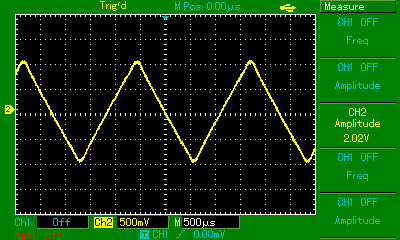
\includegraphics[width=0.7\textwidth]{dreieck.png}
  \caption{Linienspektrum einer Dreiecksschwingung.}
  \label{fig:dreieck_synthese}
\end{figure}
\begin{table}
  \centering
  \begin{tabular}{c c c c}
    \toprule
    Nummer der Oberwelle & $U_\text{e}$ in \si{\volt} &
    $U_\text{theo}$ in \si{\volt} & relative Abweichung in \% \\
    \midrule
    1 & 0.609 & 0.609 & 0.00 \\
    3 & 0.067 & 0.067 & 0.00 \\
    5 & 0.024 & 0.024 & 0.00 \\
    7 & 0.012 & 0.012 & 0.00 \\
    9 & 0.008 & 0.008 & 0.00 \\
    \bottomrule
  \end{tabular}
  \caption{Vergleich von eingestellten und berechneten Werten für die Amplituden
    der Koeffizienten bei der Synthese der Dreieckschwingung.}
  \label{tab:synthese_dreieck}
\end{table}
